% Chapter Template

\chapter{Problem Solution} % Main chapter title

\label{Chapter6} % Change X to a consecutive number; for referencing this chapter elsewhere, use \ref{ChapterX}

\lhead{Chapter 6. \emph{Problem Solution}} % Change X to a consecutive
% number; this is for the header on each page - perhaps a shortened title

%----------------------------------------------------------------------------------------
%	SECTION 1
%----------------------------------------------------------------------------------------

\section{Integrate Henshin with DPF}

DPF is a a framework where it is possible to create an arbitrary levels of
metamodels, and that gives the users the freedom to define a well formed domain
specific modeling language with support for creating an unlimited number of
metamodels and to define constraints for each specification at each level. The
framework provides the possibility to define specifications that specify
underlying specifications. Where each specification
$\spec{S}$\textsubscript{n+1} defines the abstract syntax for a specification
$\spec{S}$\textsubscript{n}. For DPF to be a framework that follows the visions
of model driven engineering it needs to have support for automation of
specifications over different levels of abstraction. It already has support for
some cases of model transformations. There is one natural model transformation
for DPF when specifying a new specification. A new specification will always
be specified by a modeling language that corresponds to a specification
$\spec{S}$\textsubscript{n+1}. These specification may either be a user created
specification or the default specification provided by the framework, that
conforms to it self. The creation of a new specification can be viewed as the
first support for automation over levels of abstraction for models that the
Diagram Predicate Framework provides. In 2012 Anders Sandven published his
master thesis\cite{Sandven_thesis}, where he implemented support for generating
source code with the DPF Editor. DPF does not provide support for applying an
exogenous model transformation to a specification described in one domain
specific modeling language to a model expressed in another domain specific
modeling language. To achieve this we want to integrate Henshin transformation
language\cite{Arendt2010} to the framework.  

\begin{figure}[H]
	\centering
	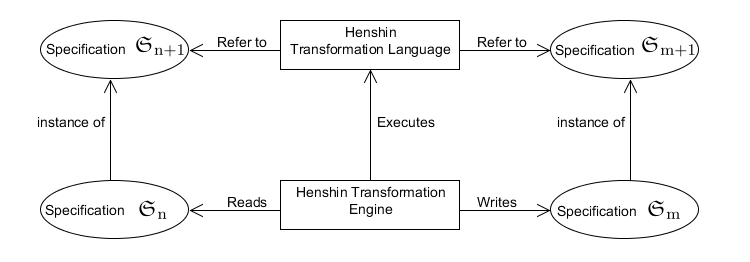
\includegraphics[scale=0.7]{./Figures/TransformationSolutionBasic.png}
	\caption[Integrating Henshin with DPF]
	{Using Henshin transformation language to translate a specification
	$\spec{S}$\textsubscript{n}.}
	\label{fig:Simple_Solution}
\end{figure}

Figure~\ref{fig:Simple_Solution} explains how we want to integrate the Henshin
transformation language, that consist of a transformation language and a
transformation engine, with DPF. We use the Henshin transformation engine to
read an instance specification $\spec{S}$\textsubscript{n} and write an instance
specification $\spec{S}$\textsubscript{m}. To achieve this the transformation
engine executes a set of transformation rules written in the Henshin
Transformation Language. These transformation rules refers to both the
specification $\spec{S}$\textsubscript{n+1} and specification
$\spec{S}$\textsubscript{m+1} that the source and target model are typed over.

The problem with integrating Henshin with DPF is that Henshin is implemented by
EMF, and therefore utilize OMG's MOF. So the Henshin transformation language
only supports models that are created accordingly to the four layer metamodeling
that MOF provides. This a problem for DPF since the framework does not
utilize MOF and has support for an arbitrary level of metamodels.  

\begin{figure}[H]
	\centering
	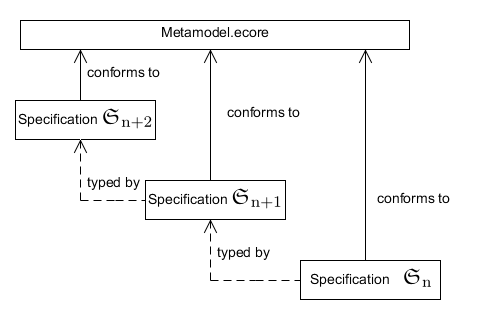
\includegraphics[scale=0.7]{./Figures/metamodelSpecification.png}
	\caption[Specification relationship with core metamodel]
	{Relationship between layers of specification.}
	\label{fig:core_metamodel}
\end{figure}

%----------------------------------------------------------------------------------------
%	SECTION 2
%----------------------------------------------------------------------------------------
\section{DPF Model Transformation Editor}







\begin{figure}[H]
	\centering
	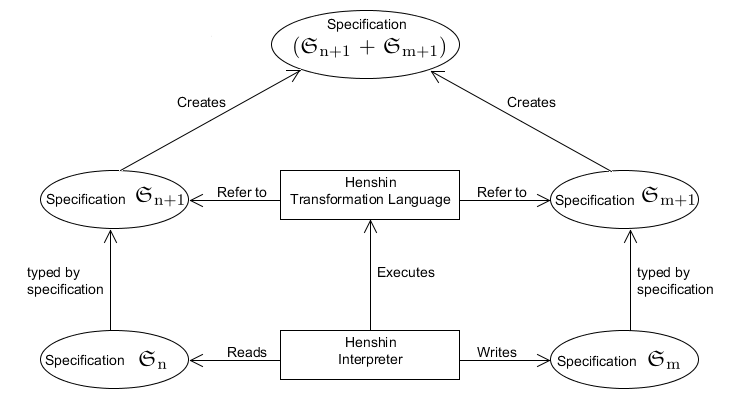
\includegraphics[scale=0.7]{./Figures/TransformationSolution_Correspond.png}
	\caption[Specification for the correspondence objects]
	{The solution expanded with a specification for the correspondence objects.}
	\label{fig:Solution_CorrespondanceObjects}
\end{figure}



\section{Henshin Metamodel}

\begin{figure}[H]
	\centering
	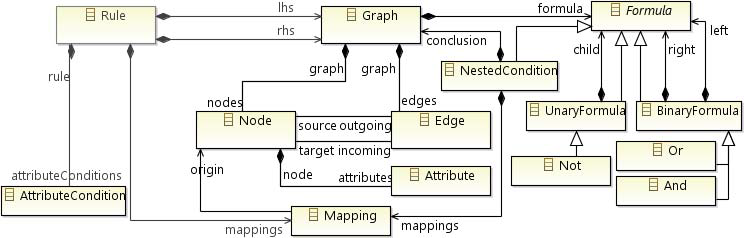
\includegraphics[scale=0.8]{./Figures/Henshin_metamodel.png}
	\caption[Henshin transformation meta-model]
	{Henshin transformation meta-model\cite{Arendt2010}.}
	\label{fig:Henshin_metamodel}
\end{figure}

A \textbf{Rule} in Henshin represents a new transformation rule that has a name,
a description and three properties. The first property disables or enables the
transformation rule, while the two other properties lets the user enable or
disable injective matching and the check dangling condition. The rule class
works as the root for all other elements present in
figure~\ref{fig:Henshin_metamodel}. A new rule defines a left hand side and a
right hand side \textbf{Graph}. The content of the LHS graph represents the
model pattern used to locate matches in an instance graph while the RHS
represents the model pattern that replaces the LHS. 



\section{Integrateing Henshin with DPF Model Transformation Editor}

\section{Henhsin Editor}



